\begin{frame}
\frametitle{Electronic Flight Bags}
\begin{center}
Aeronautical Data and Information
\end{center}
\end{frame}

\begin{frame}
\frametitle{Aeronautical Data and Information}
\begin{block}{Aviation, Navigation and Geodesy}
\begin{itemize}
\item<1-> I have not taken any serious programming steps toward solving this problem.
\item<2-> This stuff gets me a bit ranty.
\item<3-> Here is the problem.
\end{itemize}
\end{block}
\end{frame}

\begin{frame}
\frametitle{CASR 175}
\begin{block}{What is CASR 175 about?}
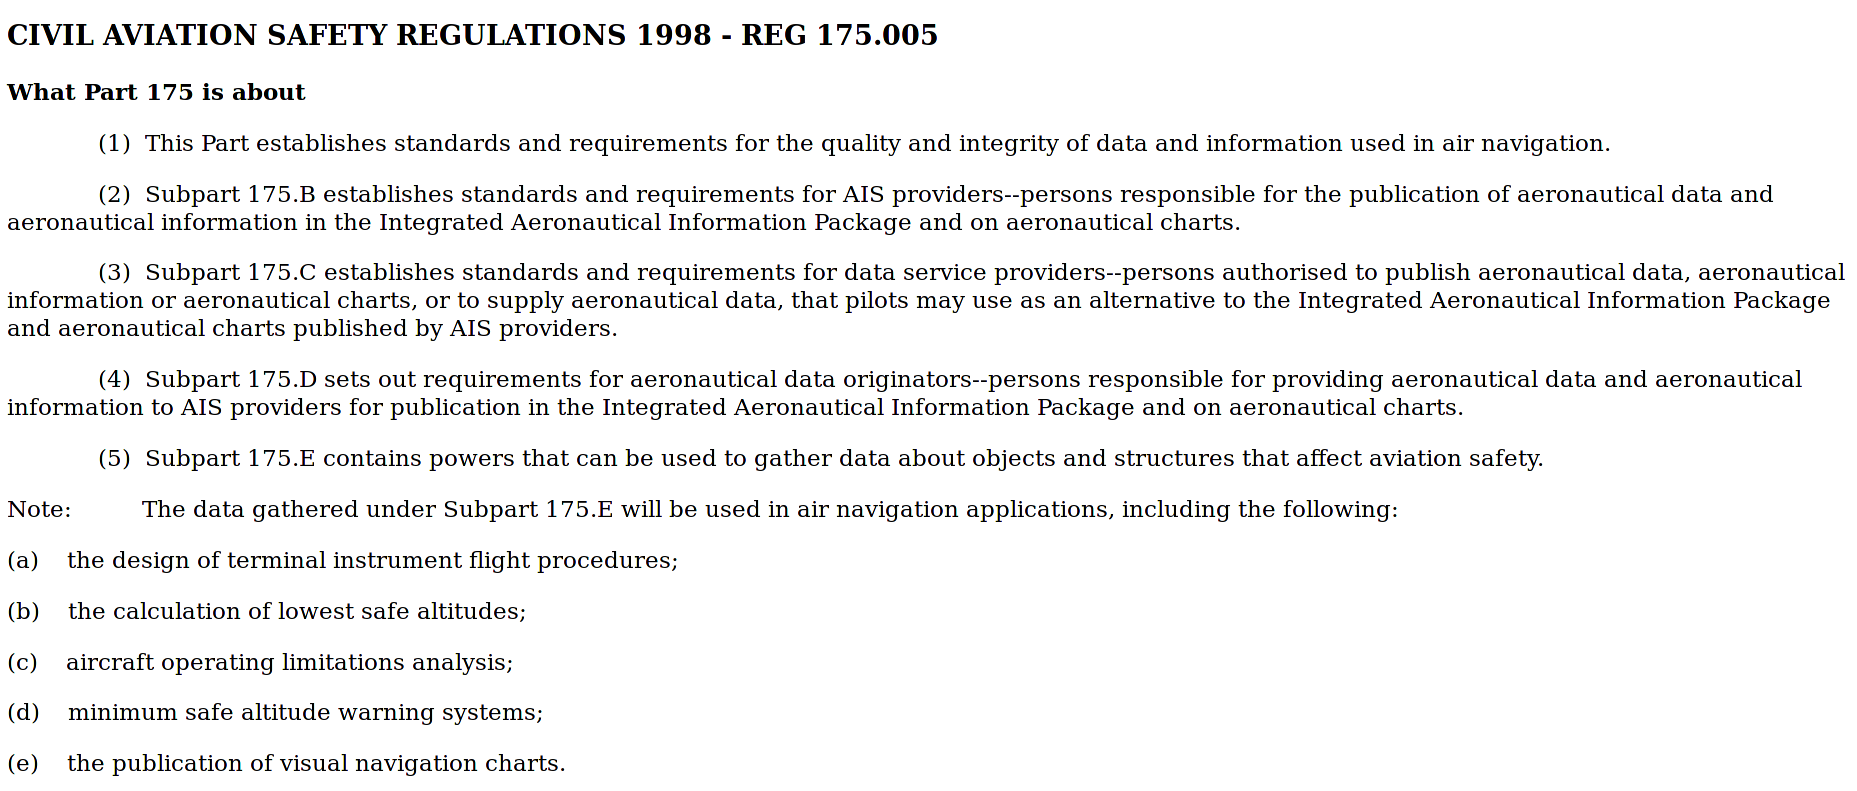
\includegraphics[height=0.5\textheight]{image/casr175_005.png}
\end{block}
\par
``(e) the publication of visual navigation charts.''
\end{frame}

\begin{frame}
\frametitle{CAR 233 (1)(h) \emph{moved to CASR 175}}
\scriptsize
\begin{block}{CAR 233 (1)(h)}
The pilot in command of an aircraft must not commence a flight if he or she has not received evidence, and taken such action as is necessary to ensure, that:
\par
\ldots
\par
(h)  the aeronautical data and aeronautical information mentioned in subregulation (1A) is carried in the aircraft and is readily accessible to the flight crew.
\end{block}
\par
\end{frame}

\begin{frame}
\frametitle{VTC/VNC}
\begin{block}{This is a Brisbane Visual Terminal Chart (VTC)}
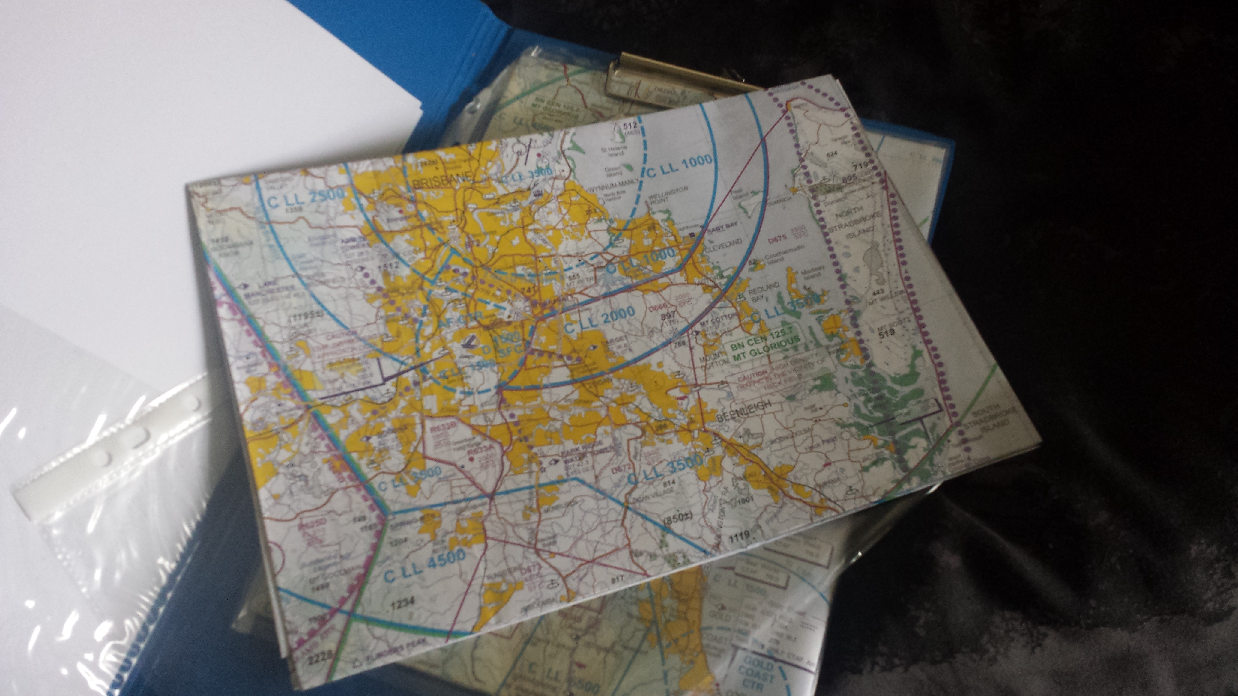
\includegraphics[height=0.3\textheight]{image/vtc.png}
\begin{itemize}
\item<1-> It unfolds out to 500mm x 1000mm.
\item<2-> Updated every 3 months (approx).
\item<3-> Similar to another chart; VNC.
\end{itemize}
\end{block}
\end{frame}

\begin{frame}
\frametitle{VTC/VNC}
\begin{block}{Under CAR 133(1)(h)}
\begin{itemize}
\item<1-> I am required to carry these charts on \emph{every flight}.
\item<2-> I don't \emph{actually} read them, because it is physically impossible in-flight.
\item<3-> I do, however, memorise the important parts.
\end{itemize}
\end{block}
\end{frame}

\begin{frame}
\frametitle{VTC/VNC}
\begin{block}{Surely these exist in electronic format?}
Why yes, they do.
\end{block}
\end{frame}

\begin{frame}
\frametitle{VTC/VNC}
\large
\begin{center}
but
\end{center}
\end{frame}

\begin{frame}
\frametitle{CASR 175.145(1)}
\begin{block}{AIS providers--publication of aeronautical charts relating to areas etc. outside authority}
(1) This regulation applies if an AIS provider publishes an aeronautical chart that includes aeronautical data or aeronautical information that relates to an area, aerodrome, airspace or ATS route not covered by the provider's certificate.
\end{block}
\end{frame}

\begin{frame}
\frametitle{CASR 175.145(1)}
\large
\begin{center}
No problem.
\par
I will use approved electronic AIS aeronautical charts.
\end{center}
\end{frame}

\begin{frame}
\frametitle{CASR 175.145(1)}
\begin{center}
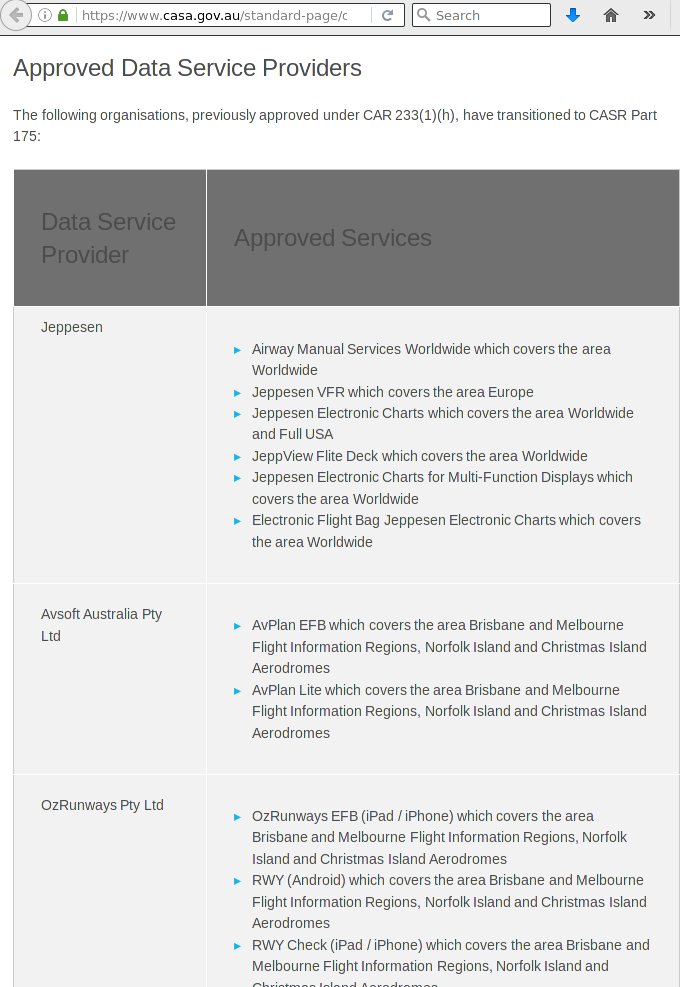
\includegraphics[height=0.8\textheight]{image/casa-approved-data-service-providers.png}
\end{center}
\end{frame}

\begin{frame}
\frametitle{CASR 175.145(1)}
\large
\begin{center}
but
\end{center}
\end{frame}

\begin{frame}
\frametitle{CASR 175.145(1)}
\large
\begin{center}
the paper charts are the authoritative data source.
\end{center}
\end{frame}

\begin{frame}
\frametitle{CASR 175.145(1)}
\begin{block}{let's fly across .png files}
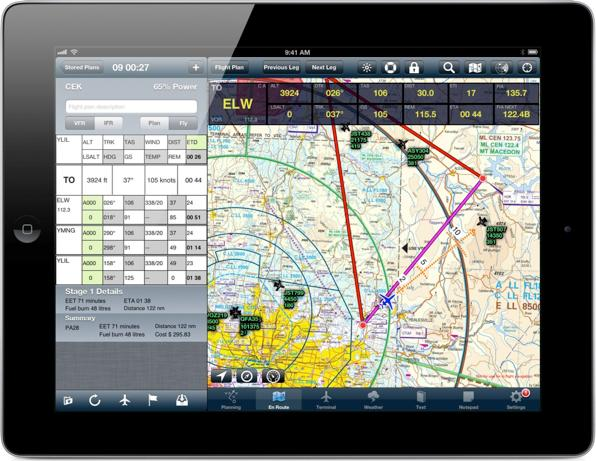
\includegraphics[height=0.5\textheight]{image/avplan-screenshot.jpg}
\end{block}
\end{frame}

\begin{frame}
\frametitle{CASR 175.145(1)}
\begin{block}{that do not georectify}
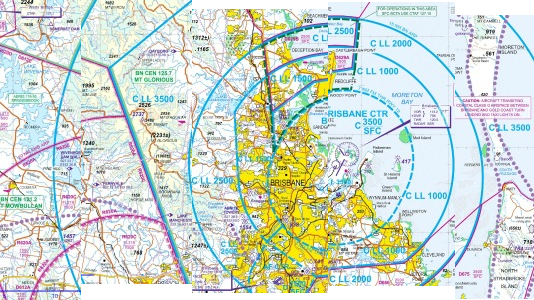
\includegraphics[height=0.5\textheight]{image/vtc-georectification.png}
\end{block}
\end{frame}

\begin{frame}
\frametitle{CASR 175.145(1)}
\begin{block}{is accuracy important?}
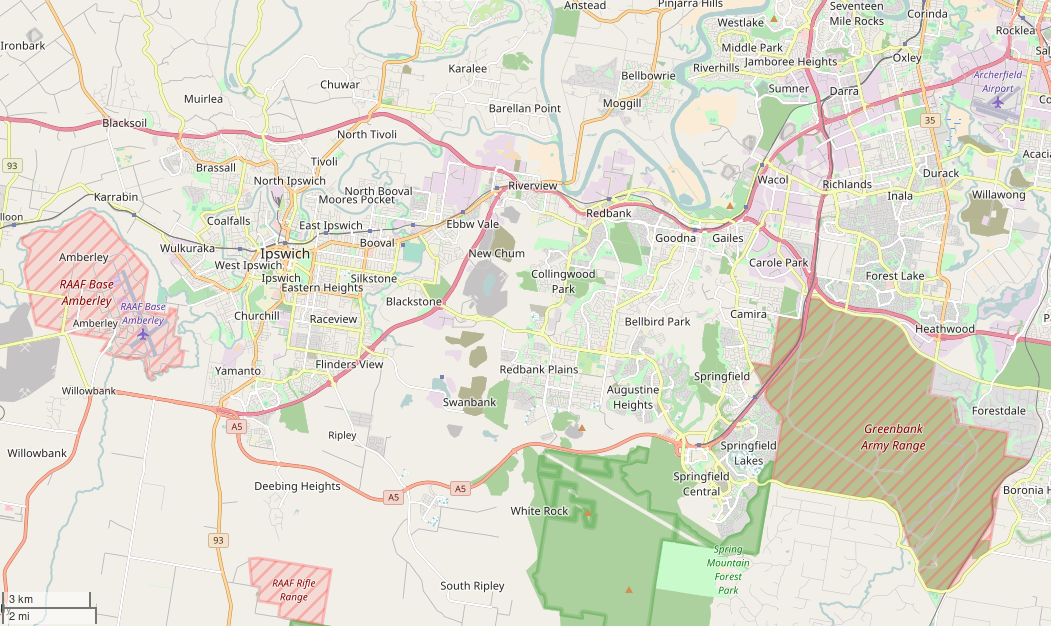
\includegraphics[height=0.5\textheight]{image/map-amberley-greenbank.png}
\end{block}
\end{frame}

\begin{frame}
\frametitle{CASR 175.145(1)}
\begin{block}{Yes}
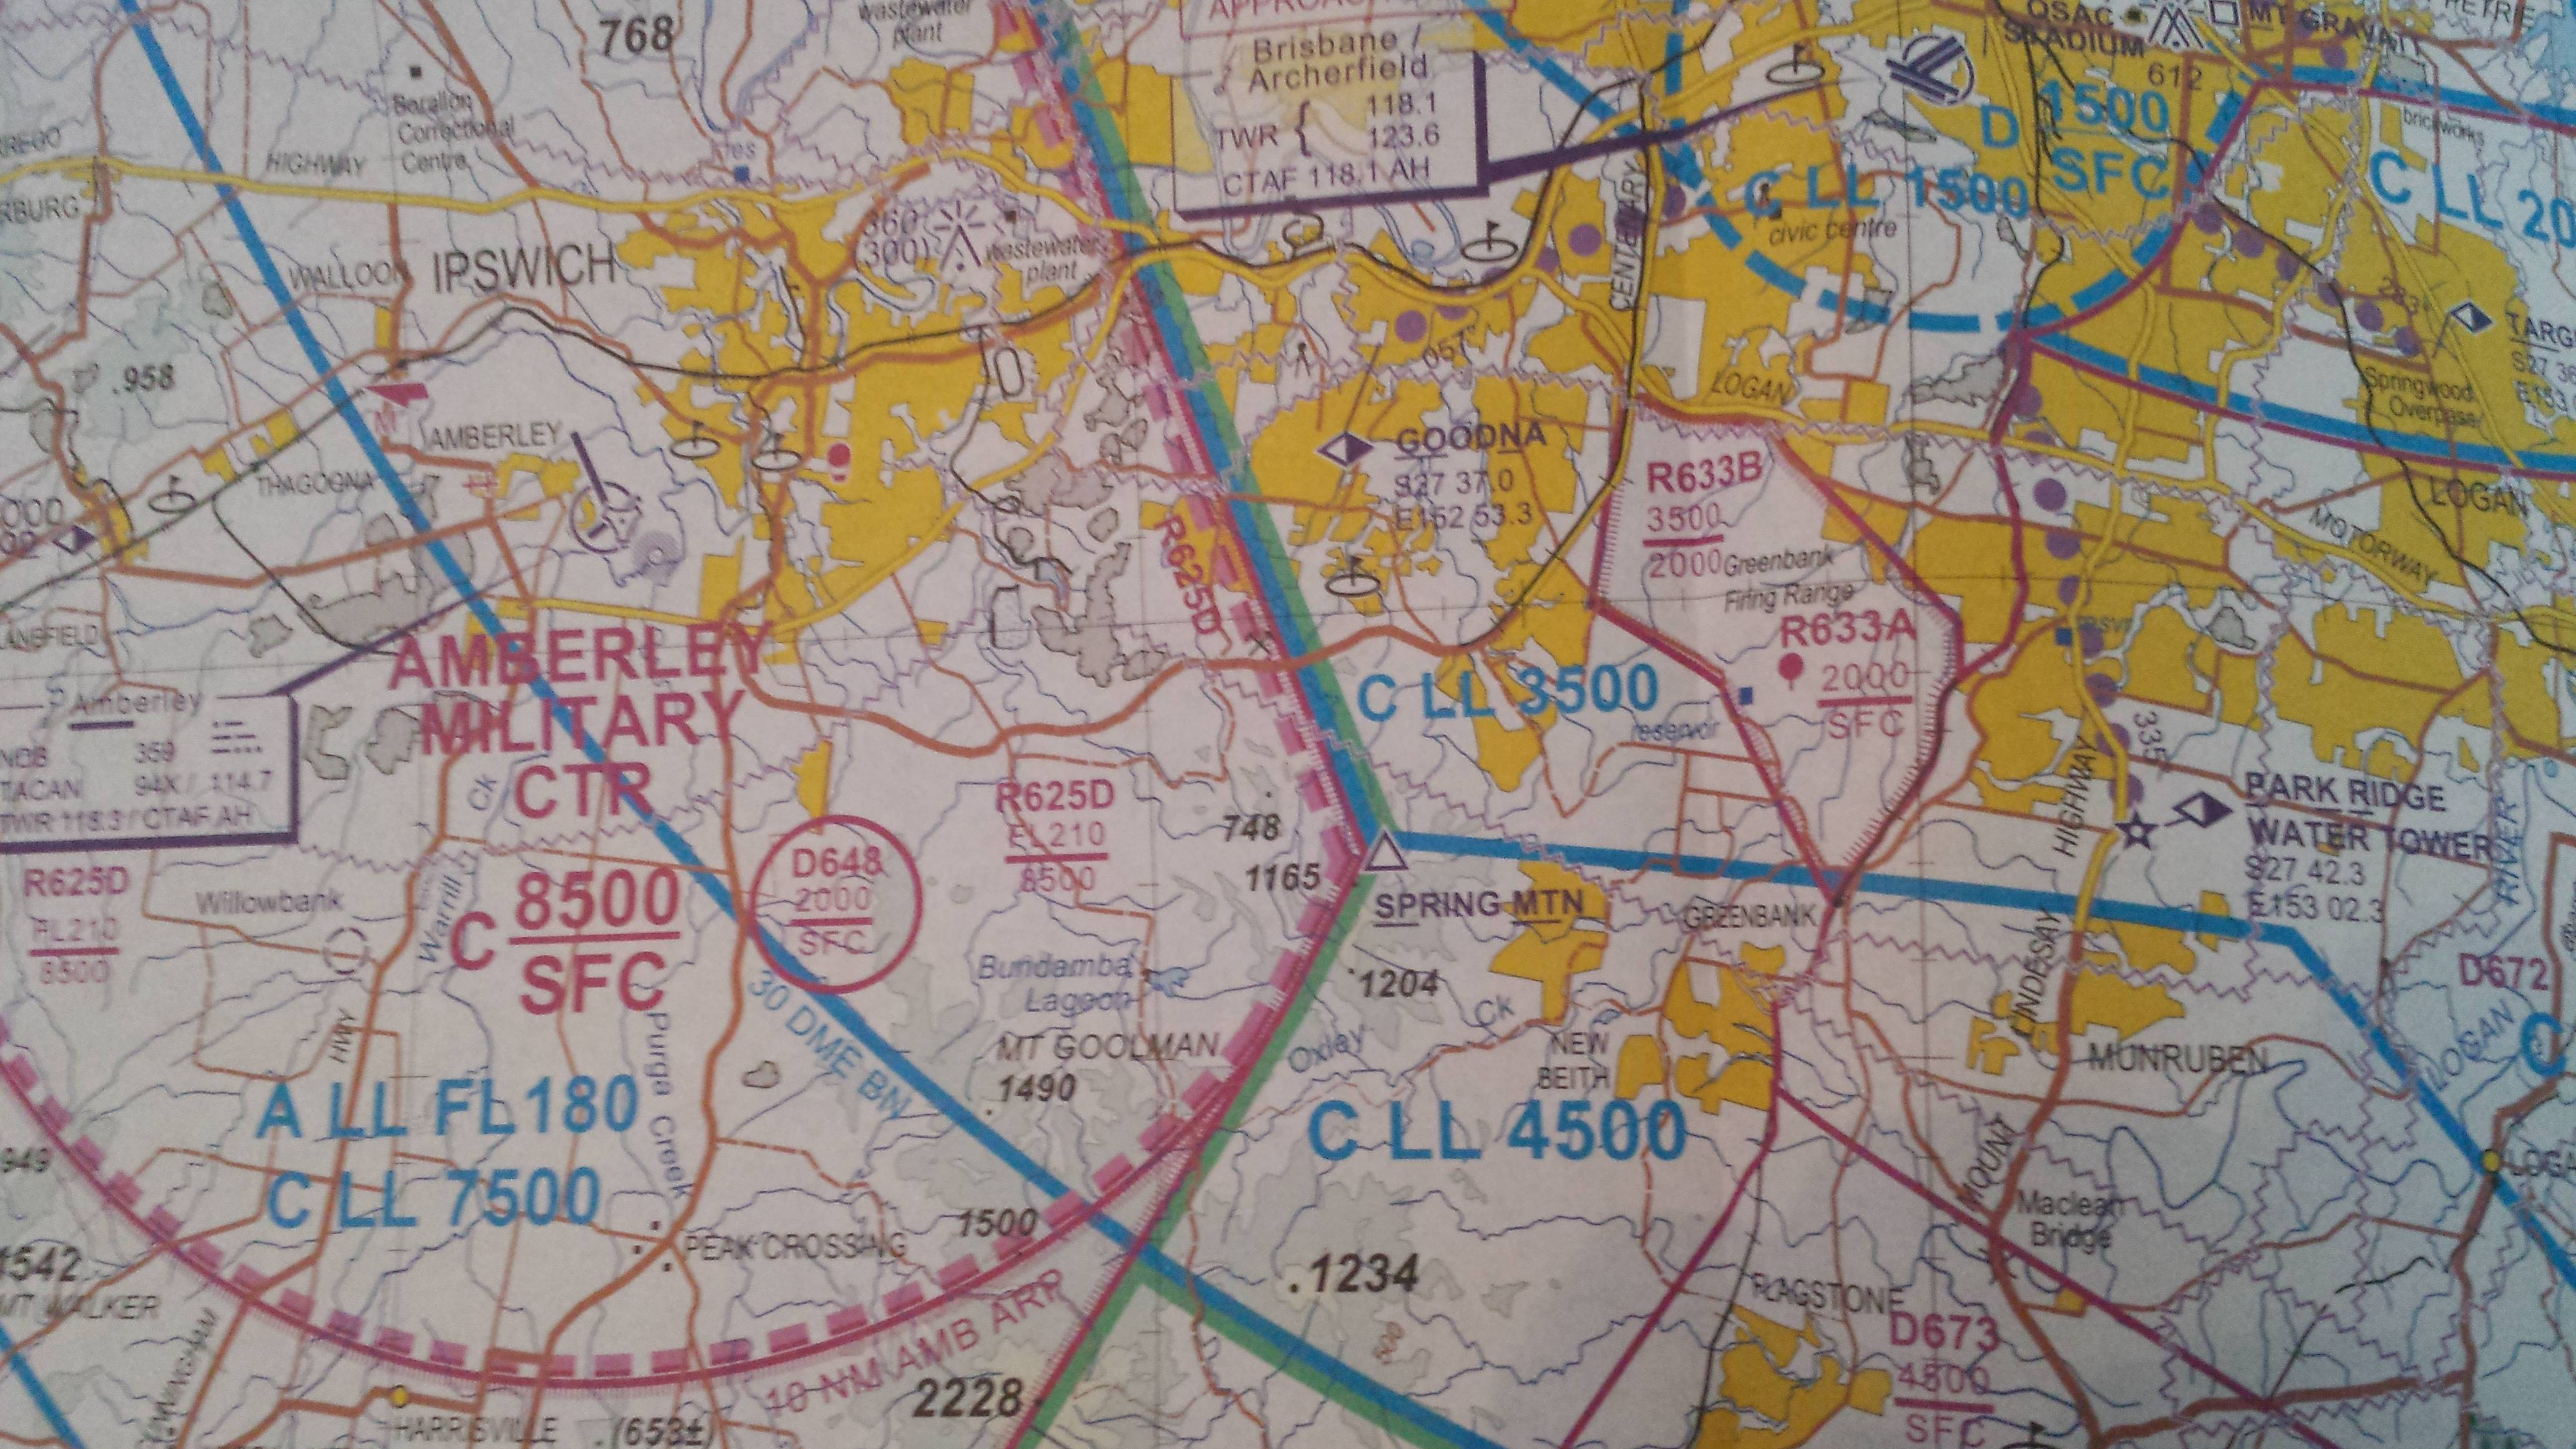
\includegraphics[height=0.5\textheight]{image/vtc-amberley-greenbank.jpg}
\begin{itemize}
\item \tiny{Amberley RAAF is \textbf{RA2}}
\item \tiny{Greenbank Army is \textbf{RA3}}
\end{itemize}
\end{block}
\end{frame}

\begin{frame}
\frametitle{CASR 175.145(1)}
\begin{block}{My nightmares are made of this stuff}
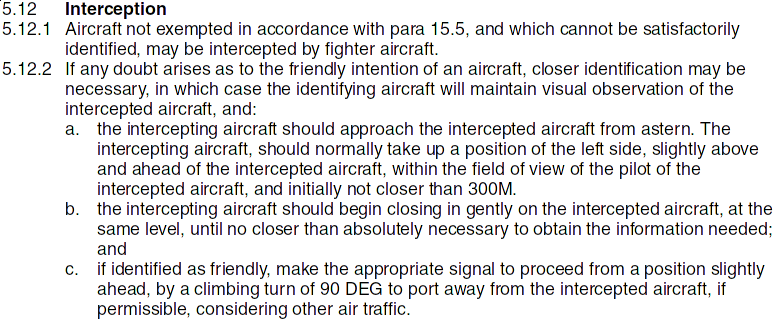
\includegraphics[height=0.5\textheight]{image/ersa-interception.png}
\end{block}
\end{frame}

\begin{frame}
\frametitle{Civil Aviation Advisory Publication 233-1}
\begin{block}{CAAP 233-1 Electronic Flight Bags \emph{(excerpt)}}
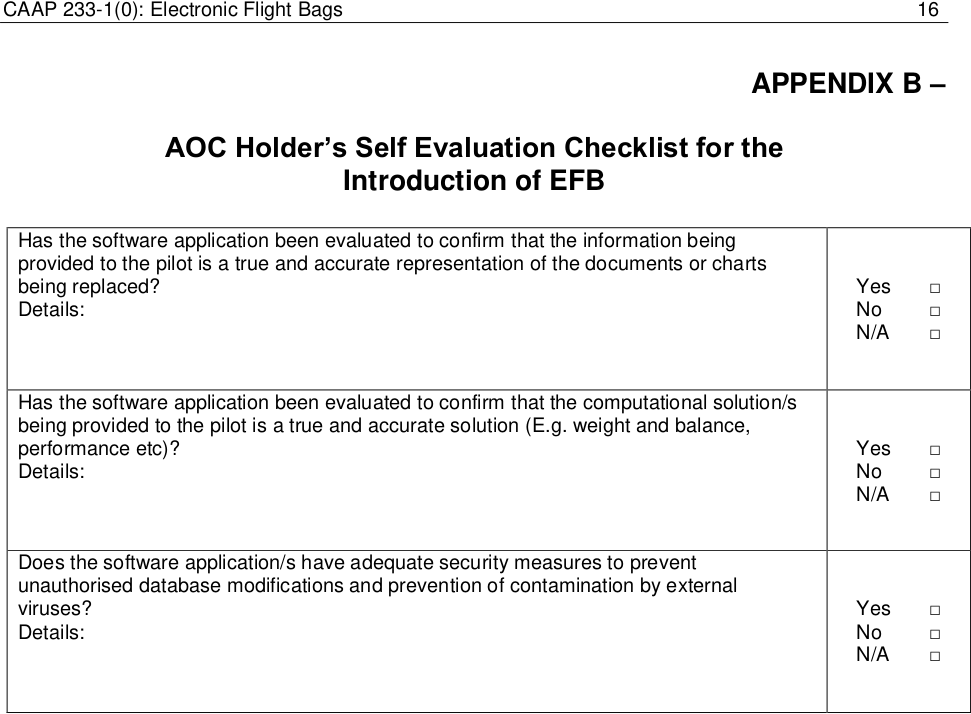
\includegraphics[height=0.6\textheight]{image/caap-233.png}
\end{block}
\end{frame}

\begin{frame}
\frametitle{CASR 175.145(1)}
\begin{center}

\includegraphics[height=0.5\textheight]{image/pls-halp.png}
\end{center}
\end{frame}
